\section{Sensoren}

\subsection{Messen der Lufttemperatur}
\subsection{Ermittlung der Niederschlagsmenge}
Dieses Unterkapitel befasst sich mit der Realisierung der Niederschlagsmessung. Diese soll nach einem Kipplöffelprinzip funktionieren und gemäss definierten Zielen eine Genauigkeit von $\pm$100 ml/$m^2$ aufweisen. Ausserdem soll als alternative zusätzlich ein Messbecher an der Wetterstation installiert werden, damit der Bauer die Niederschlagsmenge anhand einer Skala ablesen kann. In einem ersten Schritt soll das Kipplöffelprinzip näher erläutert und mit einem Selbstbau die Funktionsweise getestet werden. Anschliessend soll ein gekaufter Sensor die Wetterstation erweitern und die Implementation in der Firmware thematisiert werden. Zu guter Letzt soll die Validierung des Teilsystems folgen.
\subsubsection*{Das Kipplöffelprinzip}
Das Prinzip des Kipplöffels wird in Abbildung \ref{fig:Kipp} graphisch dargestellt.

\begin{figure}[h]
\centering
\includegraphics[width=0.8\linewidth]{graphics/Kipploeffel.png}
\caption{Darstellung des Kipplöffelprinzips}
\label{fig:Kipp}
\end{figure}

Abbildung \ref{fig:Kipp} zeigt das Kipplöffelprinzip. Der Kipplöffel (\glqq 3)\grqq) besteht im Grunde aus zwei Löffeln und ist in der Mitte drehbar mit dem Gehäuse befestigt (\glqq 4)\grqq). Regenwasser wird über eine Öffnung im Gehäusedeckel (Trichter, \glqq 1)\grqq) zum Kipplöffel befördert (\glqq 2)\grqq). Ist der Löffel mit Regenwasser gefüllt, so kippt dieser aufgrund des Gewichts und leert das Wasser über eine Öffnung im Gehäuseboden (\glqq 5)\grqq) aus. Durch die Kippung wird der andere Löffel in die Ausgangsposition bewegt und kann sich nun mit Wasser füllen. Mit der Hilfe von Reedkontakten und Magneten wird die Anzahl der Kippbewegungen gezählt. Die Niederschlagsmenge ergibt sich aus der Anzahl Kippbewegungen, multipliziert mit dem Volumen des Kipplöffels.
\newpage

\subsubsection*{Die Realisierung des Niederschlagsmengensensors}
Um die Funktionsweise des Niederschlagsmengensensors  zu testen, wird, wie im Pflichtenheft festgehalten, dieser in einem ersten Schritt selbst erstellt. Die Erstellung kann in vier Etappen unterteilt werden. Die erste Etappe ist die Erstellung des Kipplöffels. Die zweite Etappe folgt mit der Erstellung der Drehbaren Lagerung. Als dritte Etappe folgt der Trichter und die vierte und letzte Etappe widmet sich dem Gehäuse, wobei der Trichter ein Teil des Gehäuses darstellt. Das Gehäuse wird, bei verwendung der Eigenproduktion, erst im Projekt 6 mit dem Gehäuse der gesamten Wetterstation erstellt.
\paragraph{Etappe 1: Realisierung des Kipplöffels}
Wichtig für die Erstellung des Kipplöffels sind die Dimensionierung und die Materialwahl.
 
Das Material soll wetterbeständig, einfach bearbeitbar und günstig sein und eine möglichst glatte Oberfläche haben. Die möglichst glatte Oberfläche ist notwendig, damit das Wasser im Kipplöffel sich nicht an der Oberfläche festhält und somit gut abfliesst. Acrylglas erfüllt diese Bedingungen und ist in jedem Baumarkt erhältlich, weshalb es als Material gewählt wird.

Die Dimensionierung ist Abhängig von der gewählten Genauigkeit im Pflichtenheft. Damit eine Genauigkeit von $\pm$100 ml/$m^2$ erreicht werden kann, müssen beide Löffel des Kipplöffels bei genau 100 ml Fassungsvermögen kippen. Damit dies erreicht wird, kann man physikalisch die statische Gleichgewichtsbedingung aufstellen und daraus die Dimensionierung folgern. Dies ist jedoch ein sehr aufwändiger, komplizierter und zeitintensiver weg. Einfacher ist es, wenn der Kipplöffel extra zu gross dimensioniert und die Füllmenge im nachhinein justiert wird. Die Justierung erfolgt mittels einer in der Höhe verstellbaren Lagerung, sowie mit in der Höhe verstellbaren Schrauben im Gehäuseboden, welche die Neigung der Endposition des Kipplöffels beeinflusst. Ein weiterer Vorteil dieser Nachjustierung ist, dass auch eine andere Füllmenge einstellbar wäre.

\begin{figure}[h]
\centering
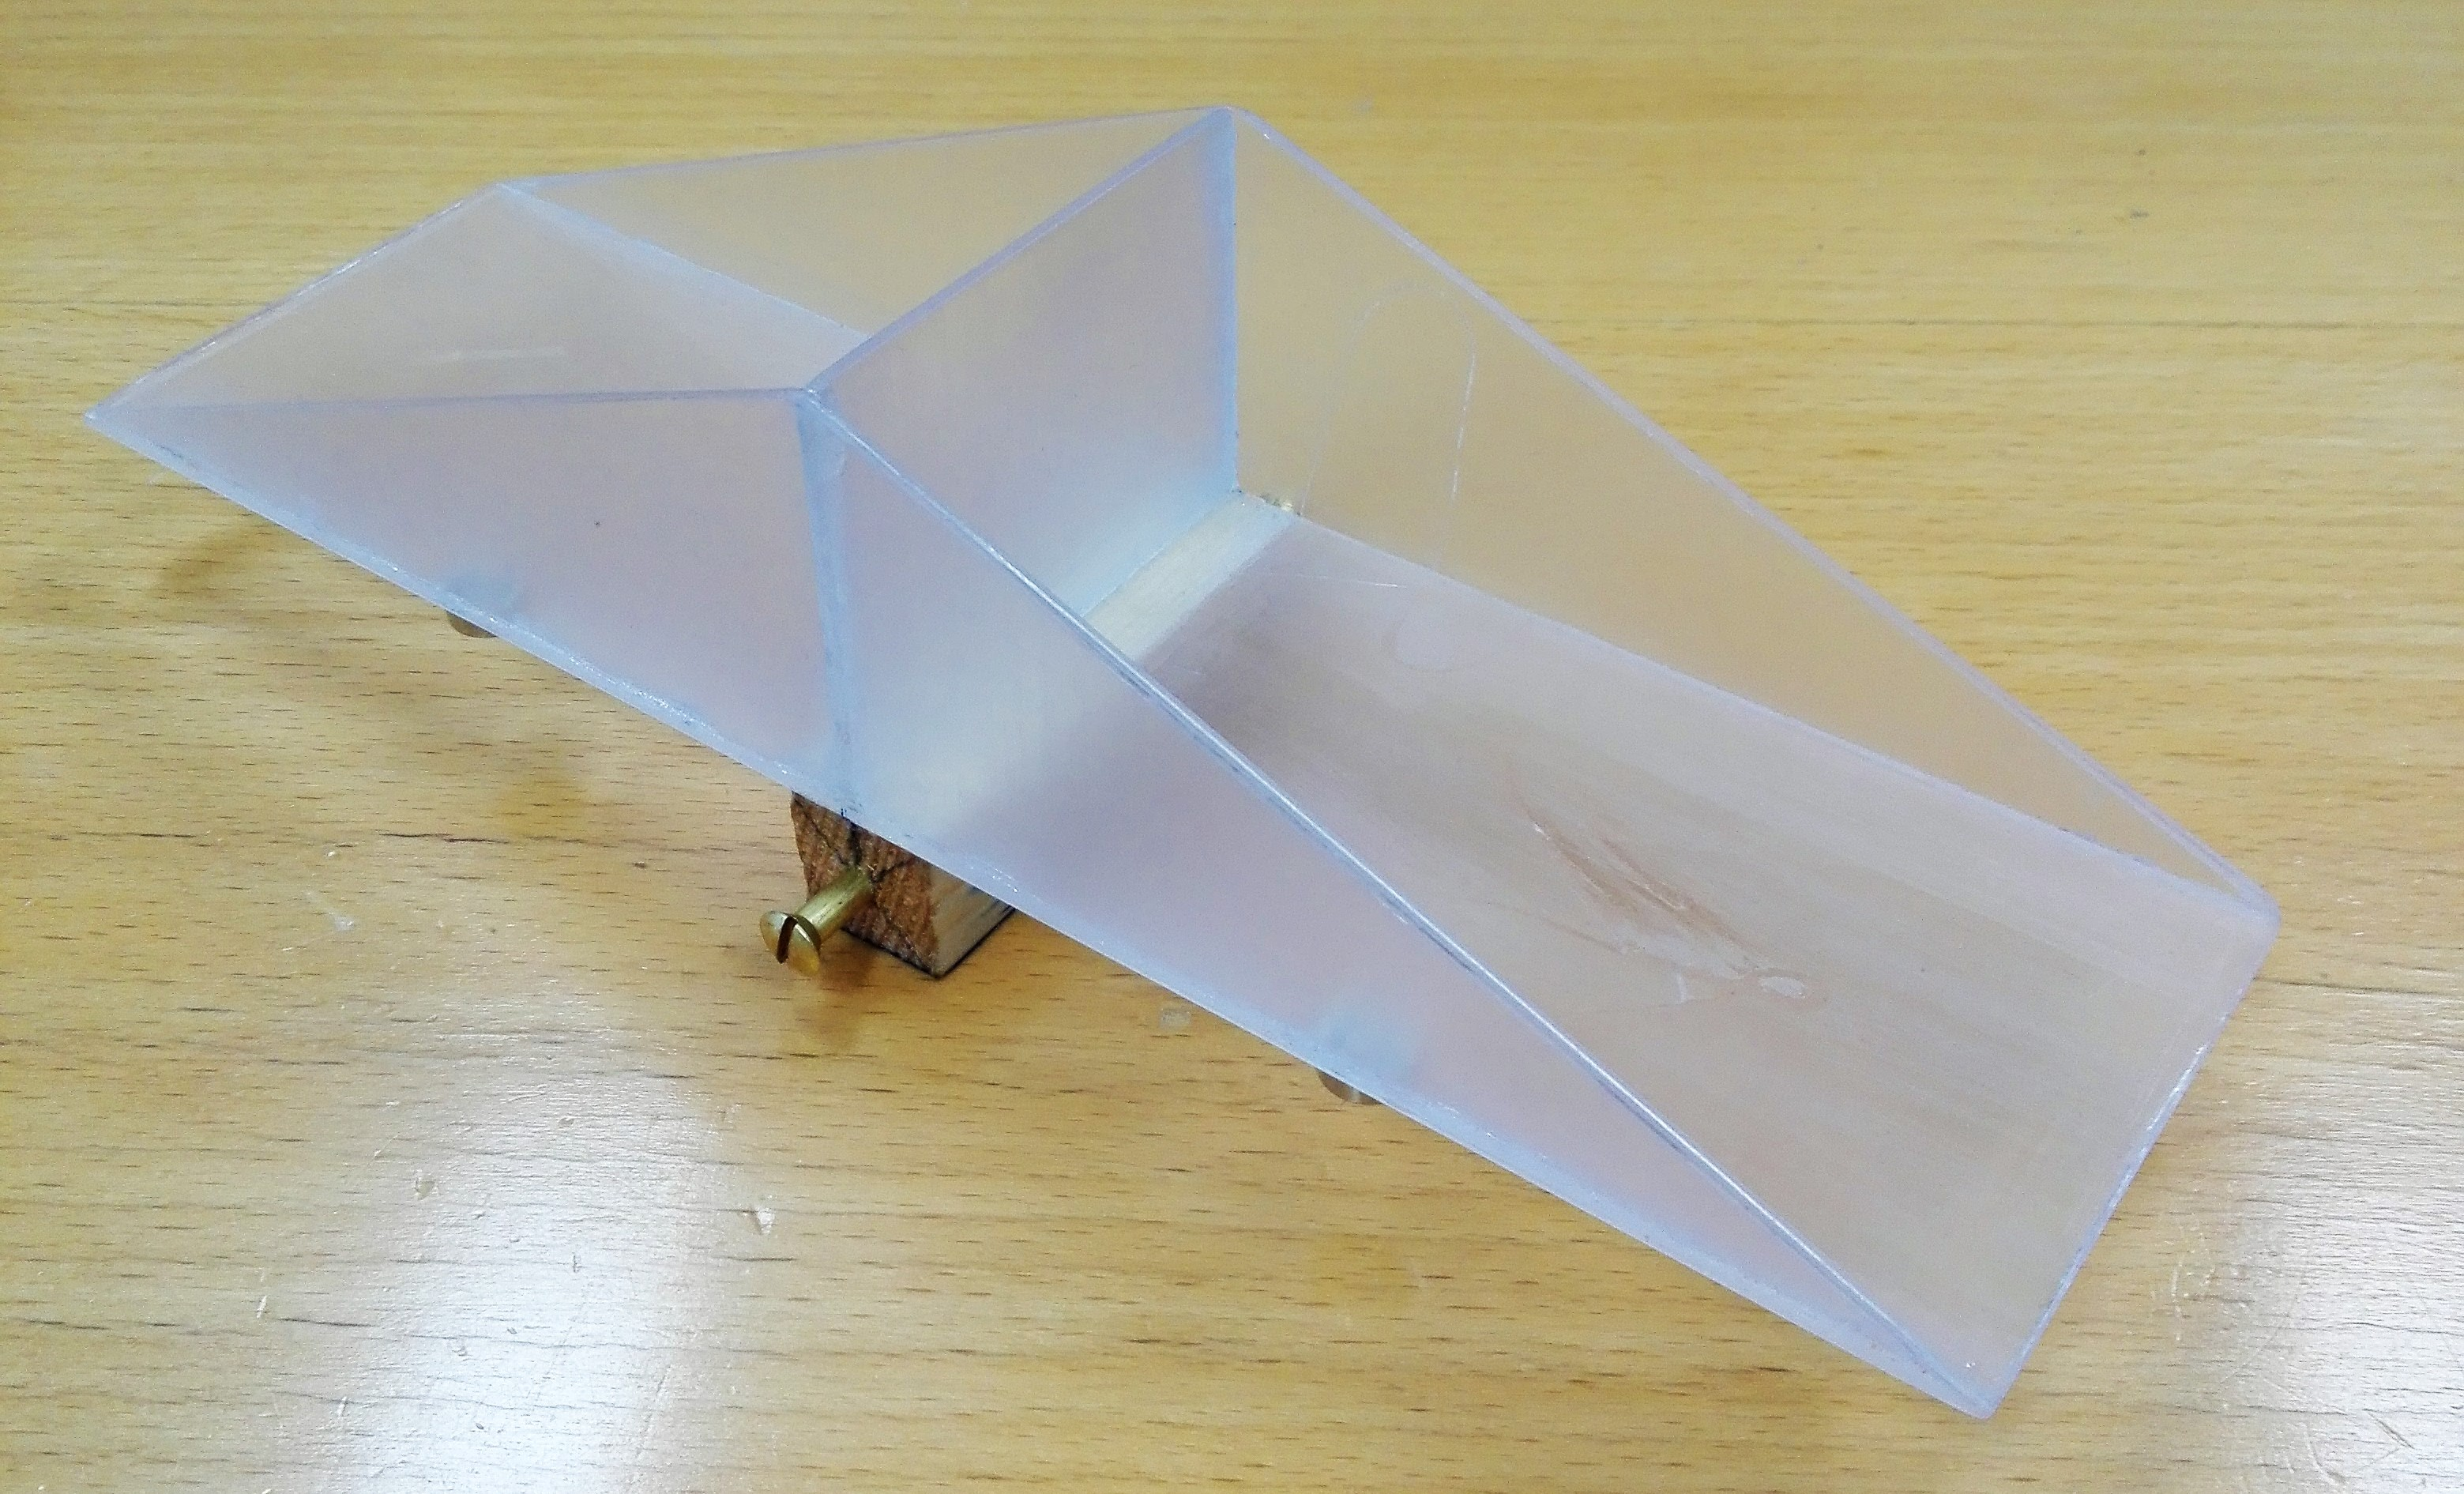
\includegraphics[width=0.8\linewidth]{graphics/Etappe1.jpg}
\caption{Selbsterstellter Kipplöffel.}
\label{fig:Etappe1}
\end{figure}

Abbildung \ref{fig:Etappe1} zeigt den selbsterstellten Kipplöffel aus Acrylglas. Die Drehachse ist mittig unter dem Kipplöffel befestigt und besteht aus einem Holzklotz mit je einer Schraube pro Seite.

\paragraph{Etappe 2: Realisierung der drehbaren Lagerung}
Die Drehbare Lagerung des Kipplöffels ist wichtig, damit der Kipplöffel auf beide Seiten kippen kann. Die Drehachse soll direkt unterhalb der Mitte des Kipplöffels befestigt sein um ein gleichmässiges Kippen zu ermöglichen. Die Höhe des Kipplöffels wird definiert durch die einstellbare Höhe der Drehachsenlagerung. 

Die Drehachse wird aus einem Stück Holz und zwei Schrauben gefertigt, wobei das Holz direkt am Kipplöffel befestigt wird. Die zwei Schrauben werden auf einem höhenverstellbarem Gerüst gelagert, so dass ein drehen möglich ist. Dieses Gerüst wird auch aus Holz gefertigt und enthält eine Metallische Fläche an der Kontaktstelle der zuvor erwähnten Schrauben, um aufkommende Reibkräfte zu verringern. Ausserdem ist dieses Gerüst höhenverstellbar über zwei mit Muttern feststellbaren Gewinden (für jede Seite eine). 

\begin{figure}[h]
\centering
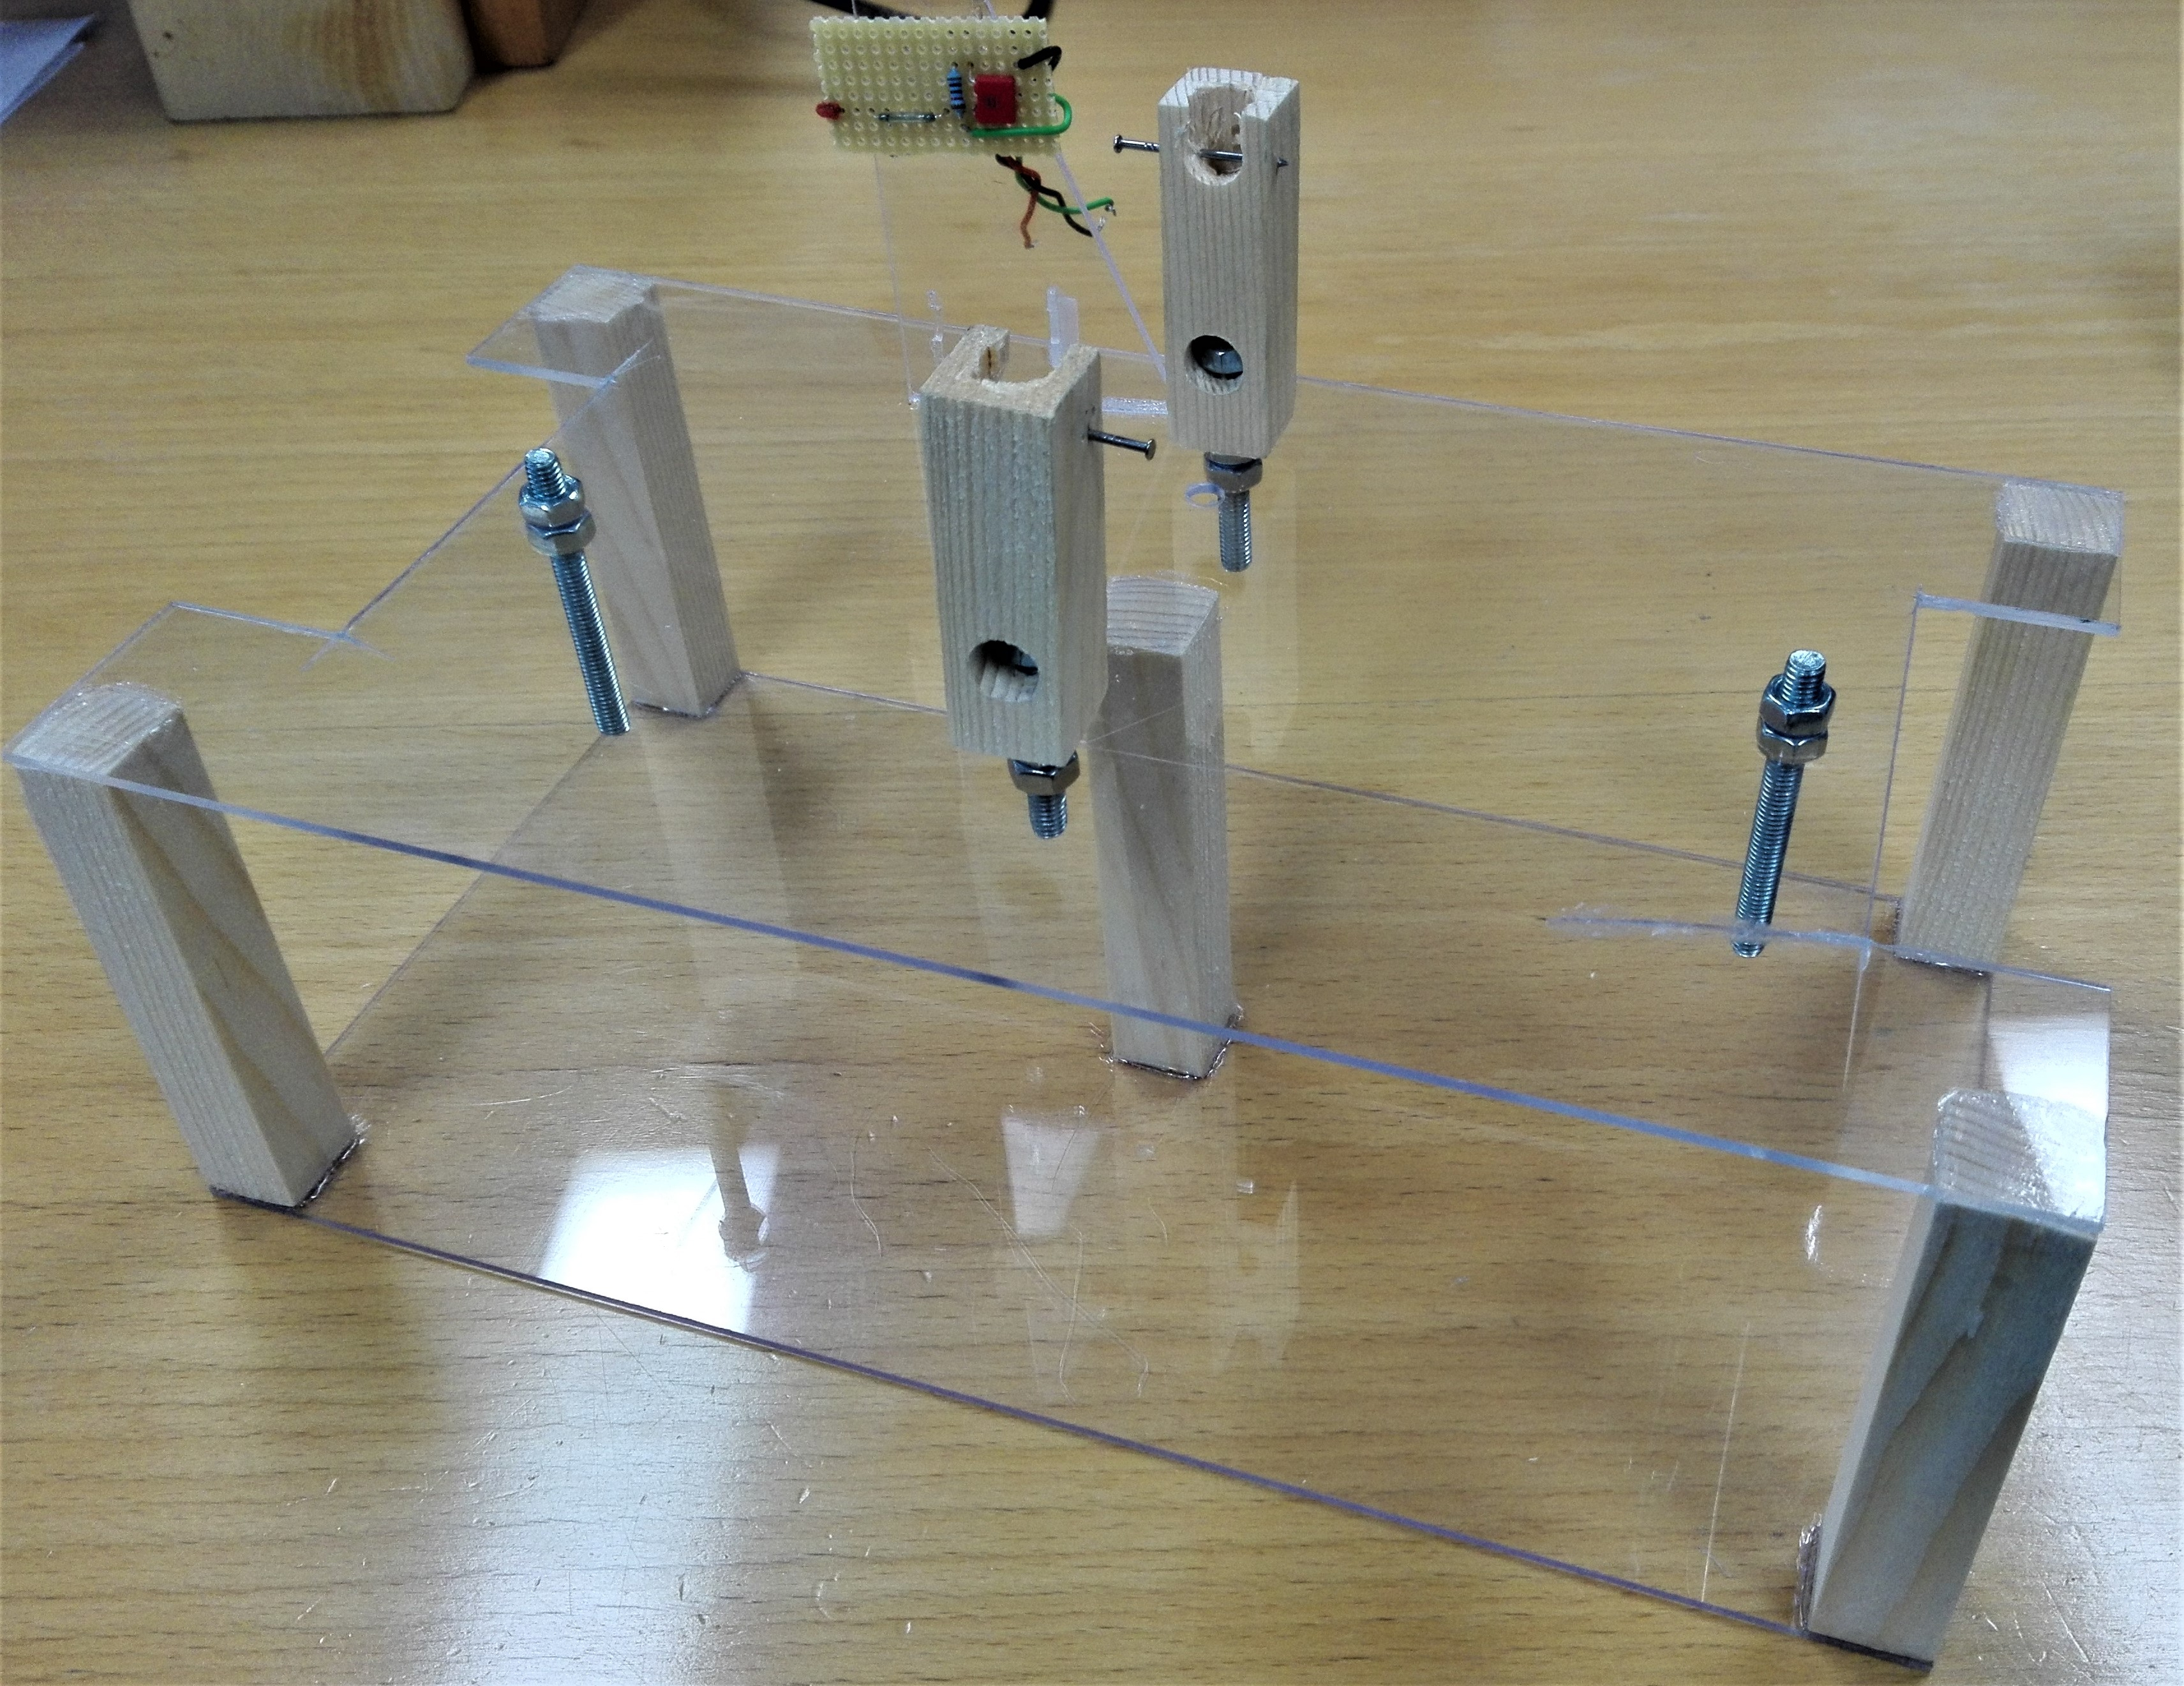
\includegraphics[width=0.8\linewidth]{graphics/Etappe2.jpg}
\caption{Selbsterstelltes Gerüst.}
\label{fig:Etappe2}
\end{figure}

Abbildung \ref{fig:Etappe2} zeigt das selbsterstellte Gerüst für die Höhenverstellbare, drehbare Lagerung des Kipplöffels. Es kann sowohl die Höhe des Kipplöffels, sowie dessen Neigung in den Endpositionen über Gewinden mit Muttern eingestellt werden. Die Schrauben des Kipplöffels kommen auf einen Stahlnagel zu liegen, womit Reibungsverluste gering gehalten werden.

\paragraph{Etappe 3: Realisierung des Trichters}
Der Trichter sorgt dafür, dass der Regen, welcher auf die Trichterfläche fällt, über der Mitte des Kipplöffels in den Löffel fliesst. Die Trichterfläche stellt gleichzeitig die Referenzfläche dar, da die gesamte Regenmenge dieser Fläche über den Kipplöffel erfasst wird. Ist diese Fläche von 1 $m^2$ abweichend, so muss in der Firmware ein Skalierungsfaktor implementiert werden, damit die Regenmenge wie gewünscht gemäss Pflichtenheft ermittelt werden kann. Der Trichter wird aus demselben Material gefertigt wie der Kipplöffel, da hier die gleichen Anforderungen gelten. Es sei angemerkt, dass der Trichter nur bei weiteren Verwendung des selbst erstellten Kipplöffels, zusammen mit dem Gehäuse der gesamten Wetterstation, erstellt wird.

\paragraph{Etappe 4: Realisierung des Gehäuses}
Das Gehäuse soll den Sensor vor ungewollten äusseren Einflüssen schützen, sowie umgebende Elektronik vor eventuellen Regenwasserspritzer. Ausserdem soll ein Schaltkreis mit Reedrelais implementiert werden, damit die Kippbewegungen von der Elektronik erfasst werden können. Es sei erwähnt, dass das Gehäuse nur bei weiteren Verwendung des selbst erstellten Sensors, zusammen mit dem Gehäuse der Wetterstation, konstruiert wird.

\paragraph{Implementierung des Schaltkreises}
Der Schaltkreis, welcher die Kippbewegungen feststellen soll, besteht im wesentlichen aus einem Reedrelais und einem Permanentmagneten. Das Reedrelais ist NO (Normally Open) und wirkt als stromkreisschliessender Schalter, sobald ein magnetisches Feld (z.B. das eines Permanentmagneten) sich in unmittelbarer Nähe befindet. Der Permanentmagnet wird auf dem Kipplöffel befestigt und das Reedrelais als Gegenstück an einem Fixpunkt in der Nähe. Wichtig dabei ist, dass das Reedrelais bei den Endpositionen des Kipplöffels nicht geschlossen ist, damit der Stromkreis geöffnet ist und Strom gespart werden kann. Das Reedrelais benötigt einen seriellen Widerstand, damit bei einem schliessen des Stromkreises kein Kurzschluss auftritt. Ausserdem soll ein Kondensator parallel zum Widerstand sein, um die Speisespannung zu glätten und so ein nutzbares Signal zu erhalten. Die Speisespannung stellt den Pegel für ein schliessen des Reedrelais, und somit auch für eine Kippbewegung dar. Um die Kippbewegungen zu zählen, kann somit entweder jede steigende oder jede fallende Flanke des Signals gezählt werden.  

\begin{figure}[h]
\centering
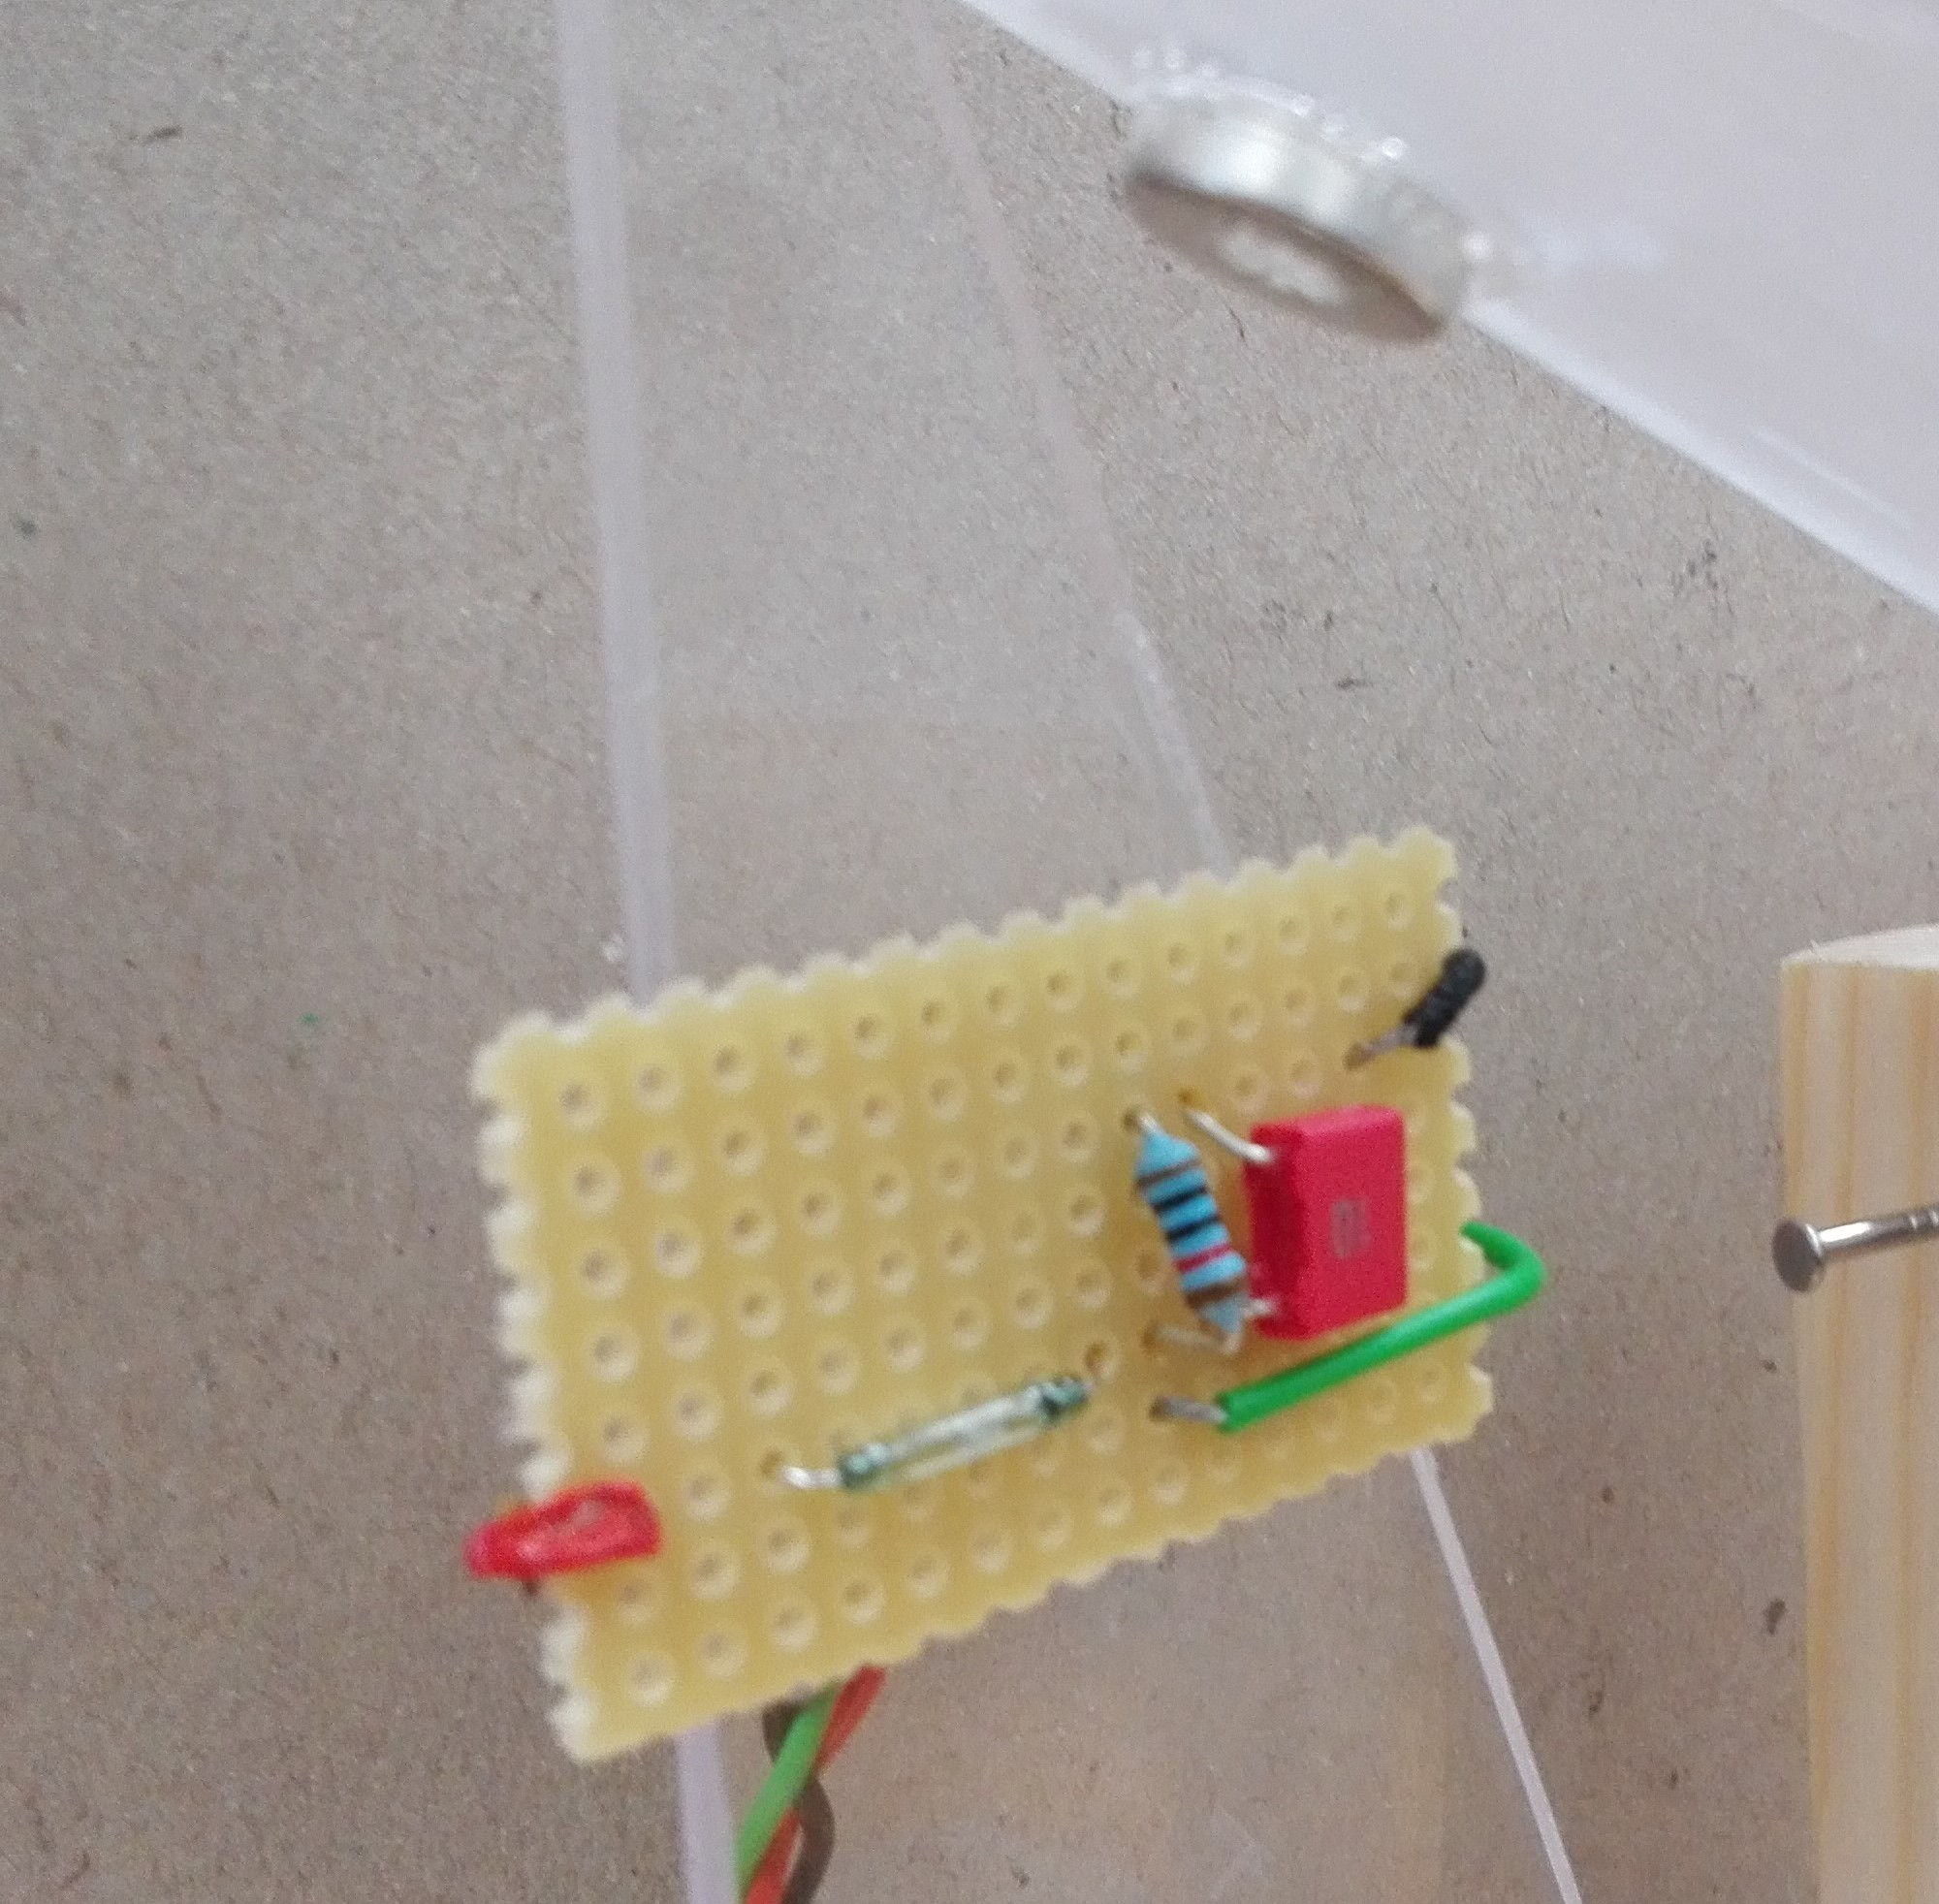
\includegraphics[width=0.4\linewidth]{graphics/KippSchalt.jpg}
\caption{Schaltkreis zur detektion der Kippbewegung.}
\label{fig:KippSchalt}
\end{figure}

Abbildung \ref{fig:KippSchalt} zeigt den Schaltkreis zur detektion der Kippbewegung. Benutzt wurde ein 10k$\Omega$ Widerstand mit einem parallel angeschlossenen 100nF Kondensator. Der Reedkontakt reagiert auf den ebenso sichtbaren Permanentmagneten, welcher an der Unterseite des Kipplöffels befestigt ist.

\paragraph{Nachteile des Selbstgebauten Niederschlagsmengensensor}
Der selbstgebaute Niederschlagssensor beweist, dass das Prinzip des Kipplöffels funktioniert. Dennoch weist der Selbstbau Mängel auf. Der verwendete Permanentmagnet muss geklebt werden, weshalb dessen Magnetfeld massiv an stärke verliert und die Schaltung deshalb äusserst nahe angebracht werden muss. Ausserdem kam es, dadurch dass keine Werkstatt zugänglich war, zu Improvisation bei nahezu allen Fertigungsschritten, was zu unkalkulierbaren Abweichungen führt. Als Beispiel sei das Spiel der drehbaren Lagerung des Kipplöffels auf dem Gerüst angeführt, was jegliche Justierungsversuche der Niederschlagsmenge beeinflusst. Aus den genannten Gründen wird vorgefertigter Sensor mit Kipplöffelprinzip verwendet.

\subsubsection*{Implentation in der Firmware}
\subsubsection*{Validierung der Niederschlagsmessung}

\newpage
\subsection{Anemometer}
\begin{minipage}{0.5\textwidth}
Für die Windgeschwindigkeitsmessung wurde ein Ersatz Anemometer von Froggit genommen.
\end{minipage}
\begin{minipage}{0.49\textwidth}
\centering
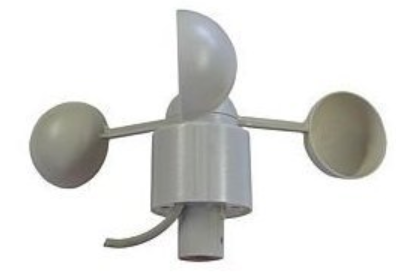
\includegraphics[width=0.7\textwidth]{graphics/Anemometer/anemometer.png}
\captionof{figure}{Anemometer \cite{AmazonAnemometer}}
\label{fig:anemometer}
\vspace{0.5cm}
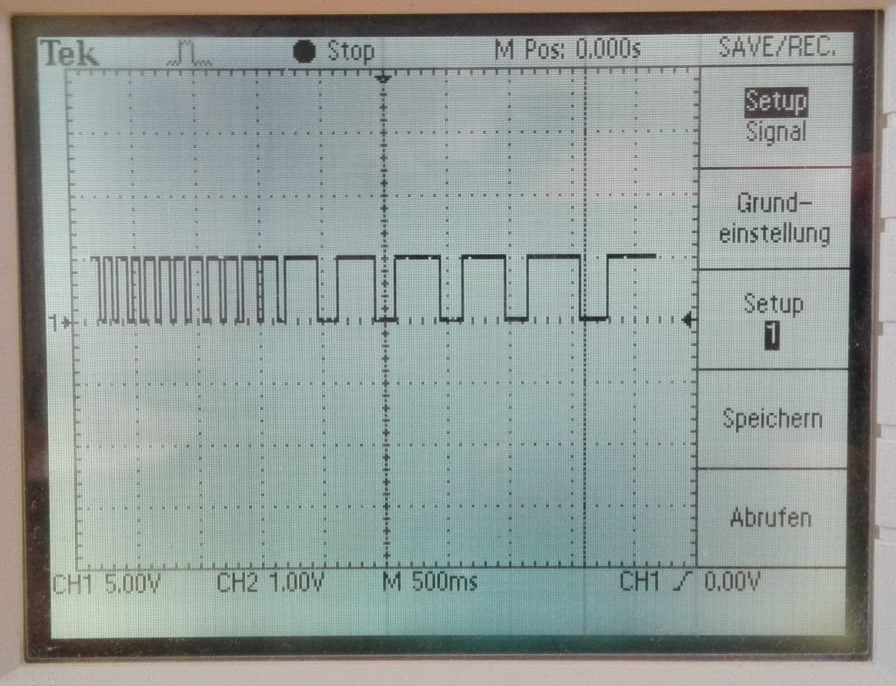
\includegraphics[width = 0.9\textwidth]{graphics/Anemometer/oszilloskop_anenometer_puls.png}
\captionof{figure}{Rechteckpulse des Anemometers.}
\label{fig:rechteckpuls_anemometer}
\end{minipage}


\subsection{Zählung der Sonnenstunden}
